\section{Hydraulics of sewer line}\label{se:hydraulics_of_sewer_line}

Methods to model hydraulics of gravity and pressurized sewer lines is explained respectively in the following. 

Modeling fluids is almost always done by considering it as a control volume. The cause of this is that it is rarely efficient, computational wise, or possible to consider the individual fluid particles.
Henceforth the control volume will be denoted by the letter $\Omega$ which will correspond to some amount of fluid in a length of sewer line.

The open channel flow in gravity sewer lines can be described by the Saint-Venant equations which gives an expression for conservation of mass and momentum.
Some assumptions is made when utilizing the Saint-Venant equations:

\begin{table}[H]
\begin{enumerate}
\item The flow in the channel is one dimensional and as such any curvature of the sewer line is neglected.
\item Fluid in the sewer line is considered incompressible i.e. the pressure is assumed hydrostatic.
\item The only forces considered is friction, pressure and gravity.
\item The water height and velocity is uniform in the cross-section and only changes horizontally i.e. turbulence in the fluid is not considered.
\item The slope of the pipe bed is small
% \item The flow in the sewer is one-dimensional, meaning that the water height and velocity is uniform in the cross-section and only changes horizontally.
% \item The curvature of the sewer line is sufficiently small such that it can be considered a straight line. 
% \item Vertical accelerations is neglected and the fluid is incompressible such that the pressure can be assumed hydrostatic.
% \item The slope and the variation in width of the sewer line is small.
% \item The effect of scour and accumulation of solids are assumed to be negligible. 
\end{enumerate}
\label{tab:saintbernard_assumptions}
\end{table}

The equation for conservation of mass gives an expression for the amount of fluid flowing in to the control volume and the flow out plus the fluid stored in it.
In figure \ref{fig:firkant_kloak} a flow in a channel with vertical channel walls is shown.
%The cross section is given as $A = h \cdot B$ which both is a function of position and time.

\begin{figure}[H]
\centering
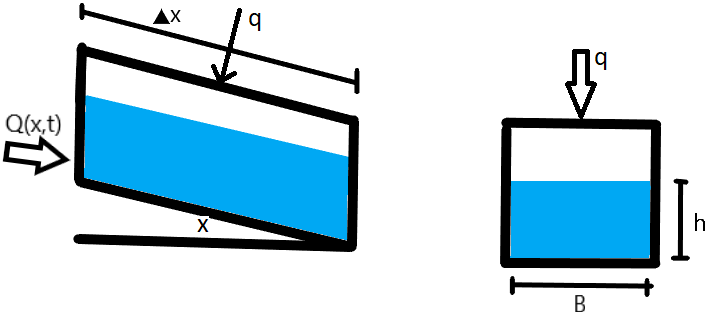
\includegraphics[width=0.45\textwidth]{report/modeling/pictures/firkant_kloak.png}
\caption{Flow in a channel with a flat bed and vertical sides where Q is flow into the channel, q is lateral flow into the channel and the cross section area is given by $\text{A} = \text{B} \cdot \text{h}$. \fxnote{Ny tegning}}
\label{fig:firkant_kloak}
\end{figure}

Flows and cross section shown in figure \ref{fig:firkant_kloak} is dependent on time and position, but in the following a simpler notation is used for an easier outline. 

The flow into the control volume is given as
\begin{equation}
	\left(Q - \frac{\partial Q}{\partial x}\cdot \frac{\Delta x}{2}\right) \cdot \Delta t + q \cdot \Delta x \cdot \Delta t
\label{flowin_saintbernard}
\end{equation}

where q is the lateral inflow into the channel and Q is the flow in the channel($\frac{m^3}{s}$. Lateral inflow could for example come from adjoint sewer pipes or a gutter drain.
The flow out of the channel is

\begin{equation}
\left(Q + \frac{\partial Q}{ \partial x} \frac{\Delta x}{2} \right) \cdot \Delta t 
\label{flowout_saintbernard}
\end{equation}

and the stored fluid in the channel is

\begin{equation}
\frac{\partial A}{\partial t}\cdot \Delta t \cdot \Delta x	
\label{stored_saintbernard}
\end{equation}

As the flow into the channel is equal to the flow out plus the change in the stored fluid in the channel, then, due to the assumption of incompressible fluid and uniformity, \ref{flowin_saintbernard}, \ref{flowout_saintbernard} and \ref{stored_saintbernard} can be combined into equation \ref{saintbernard_masse}. 

\begin{equation}
\begin{array}{l}
	\left(Q - \frac{\partial Q}{\partial x}\cdot \frac{\Delta x}{2}\right) \cdot \Delta t + q \cdot \Delta x \cdot \Delta t - \left(Q + \frac{\partial Q}{ \partial x} \frac{\Delta x}{2} \right) \cdot \Delta t - \frac{\partial A}{\partial t}\cdot \Delta t 
	\cdot \Delta x = 0 \\ 
\Updownarrow \\
q \cdot \Delta x \cdot \Delta t -\frac{\partial A}{\partial t} \cdot \Delta t 
	\cdot \Delta x - \frac{\partial Q}{\partial x} \cdot \Delta x \cdot \Delta t  = 0 
\end{array}
\label{saintbernard_masse}
\end{equation}

which can be reduced to the following by isolating and dividing with $\Delta x$ and $\Delta t$ on both sides yielding the mass conservation part of the Saint-Venant equations.
\begin{equation}	
\frac{\partial A(x,t)}{\partial t} + \frac{\partial Q(x,t)}{\partial x}=q(x,t)
\label{saintbernard_mass_lateral}
\end{equation}

For channel flows without lateral input the mass conservation is given as:
\begin{equation}	
\frac{\partial A(x,t)}{\partial t} + \frac{\partial Q(x,t)}{\partial x}=0
\label{saintbernard_mass}
\end{equation}

Momentum of the control volume $\Omega$ shown in figure \ref{fig:kloakroer} is defined as:
\begin{equation}
M(t) = m(t) \cdot v(t)
\label{eq:momentum_definition}
\end{equation}  

where M is momentum ($\frac{kg \cdot m}{s}$), m is mass ($kg$) and v is velocity($\frac{m}{s}$). Equation




\begin{figure}[H]
\centering
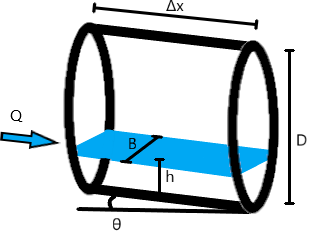
\includegraphics[width=0.45\textwidth]{report/modeling/pictures/kloakroer.png}
\caption{Sewer pipe \fxnote{Ny tegning indsæt omega i control volumet}}
\label{fig:kloakroer}
\end{figure}








\begin{equation}
	\frac{\partial Q(x,t)}{\partial t} + \frac{\partial}{\partial x} \frac{Q^2(x,t)}{A(x,t)}+ g \cdot A(x,t) (\frac{\partial h(x,t)}{\partial x} +S_f(x,t)-S_b(x)) = 0
\label{saintbernard_momentum}
\end{equation}

\begin{equation}
	S_f = \frac{Q^2n^2}{A^2R^{4/3}}
\label{Manning_formula}
\end{equation}




